% !TeX root = ../../main.tex

\section{Biomechanics of the Renal Parenchyma}

\subsection{Overview of Kidney Anatomy and Function}
\label{sec:anatomy}

% Paragraph 1: kidney is made of multiple compartments
%   - renal parenchyma
%     - cortex
%     - medulla
%   - collecting system
%   - vasculature

The human kidney, illustrated in Fig.~\ref{fig:anatomy}, is a complex organ composed of multiple compartments that work together to perform its essential functions. The renal parenchyma, which includes the cortex and medulla, is responsible for filtering blood and producing urine. The cortex, the outer layer of the kidney, contains the majority of the nephrons, the functional units of the kidney. The medulla, the inner region, consists of structures that play crucial roles in concentrating urine. The collecting system gathers urine from the nephrons and channels it into the renal pelvis, from where it flows to the bladder. Additionally, the kidney's vasculature including arteries, veins, and capillaries, supplies blood to and from the renal parenchyma, facilitating filtration and nutrient exchange.

\begin{figure}[btp]
    \centering
    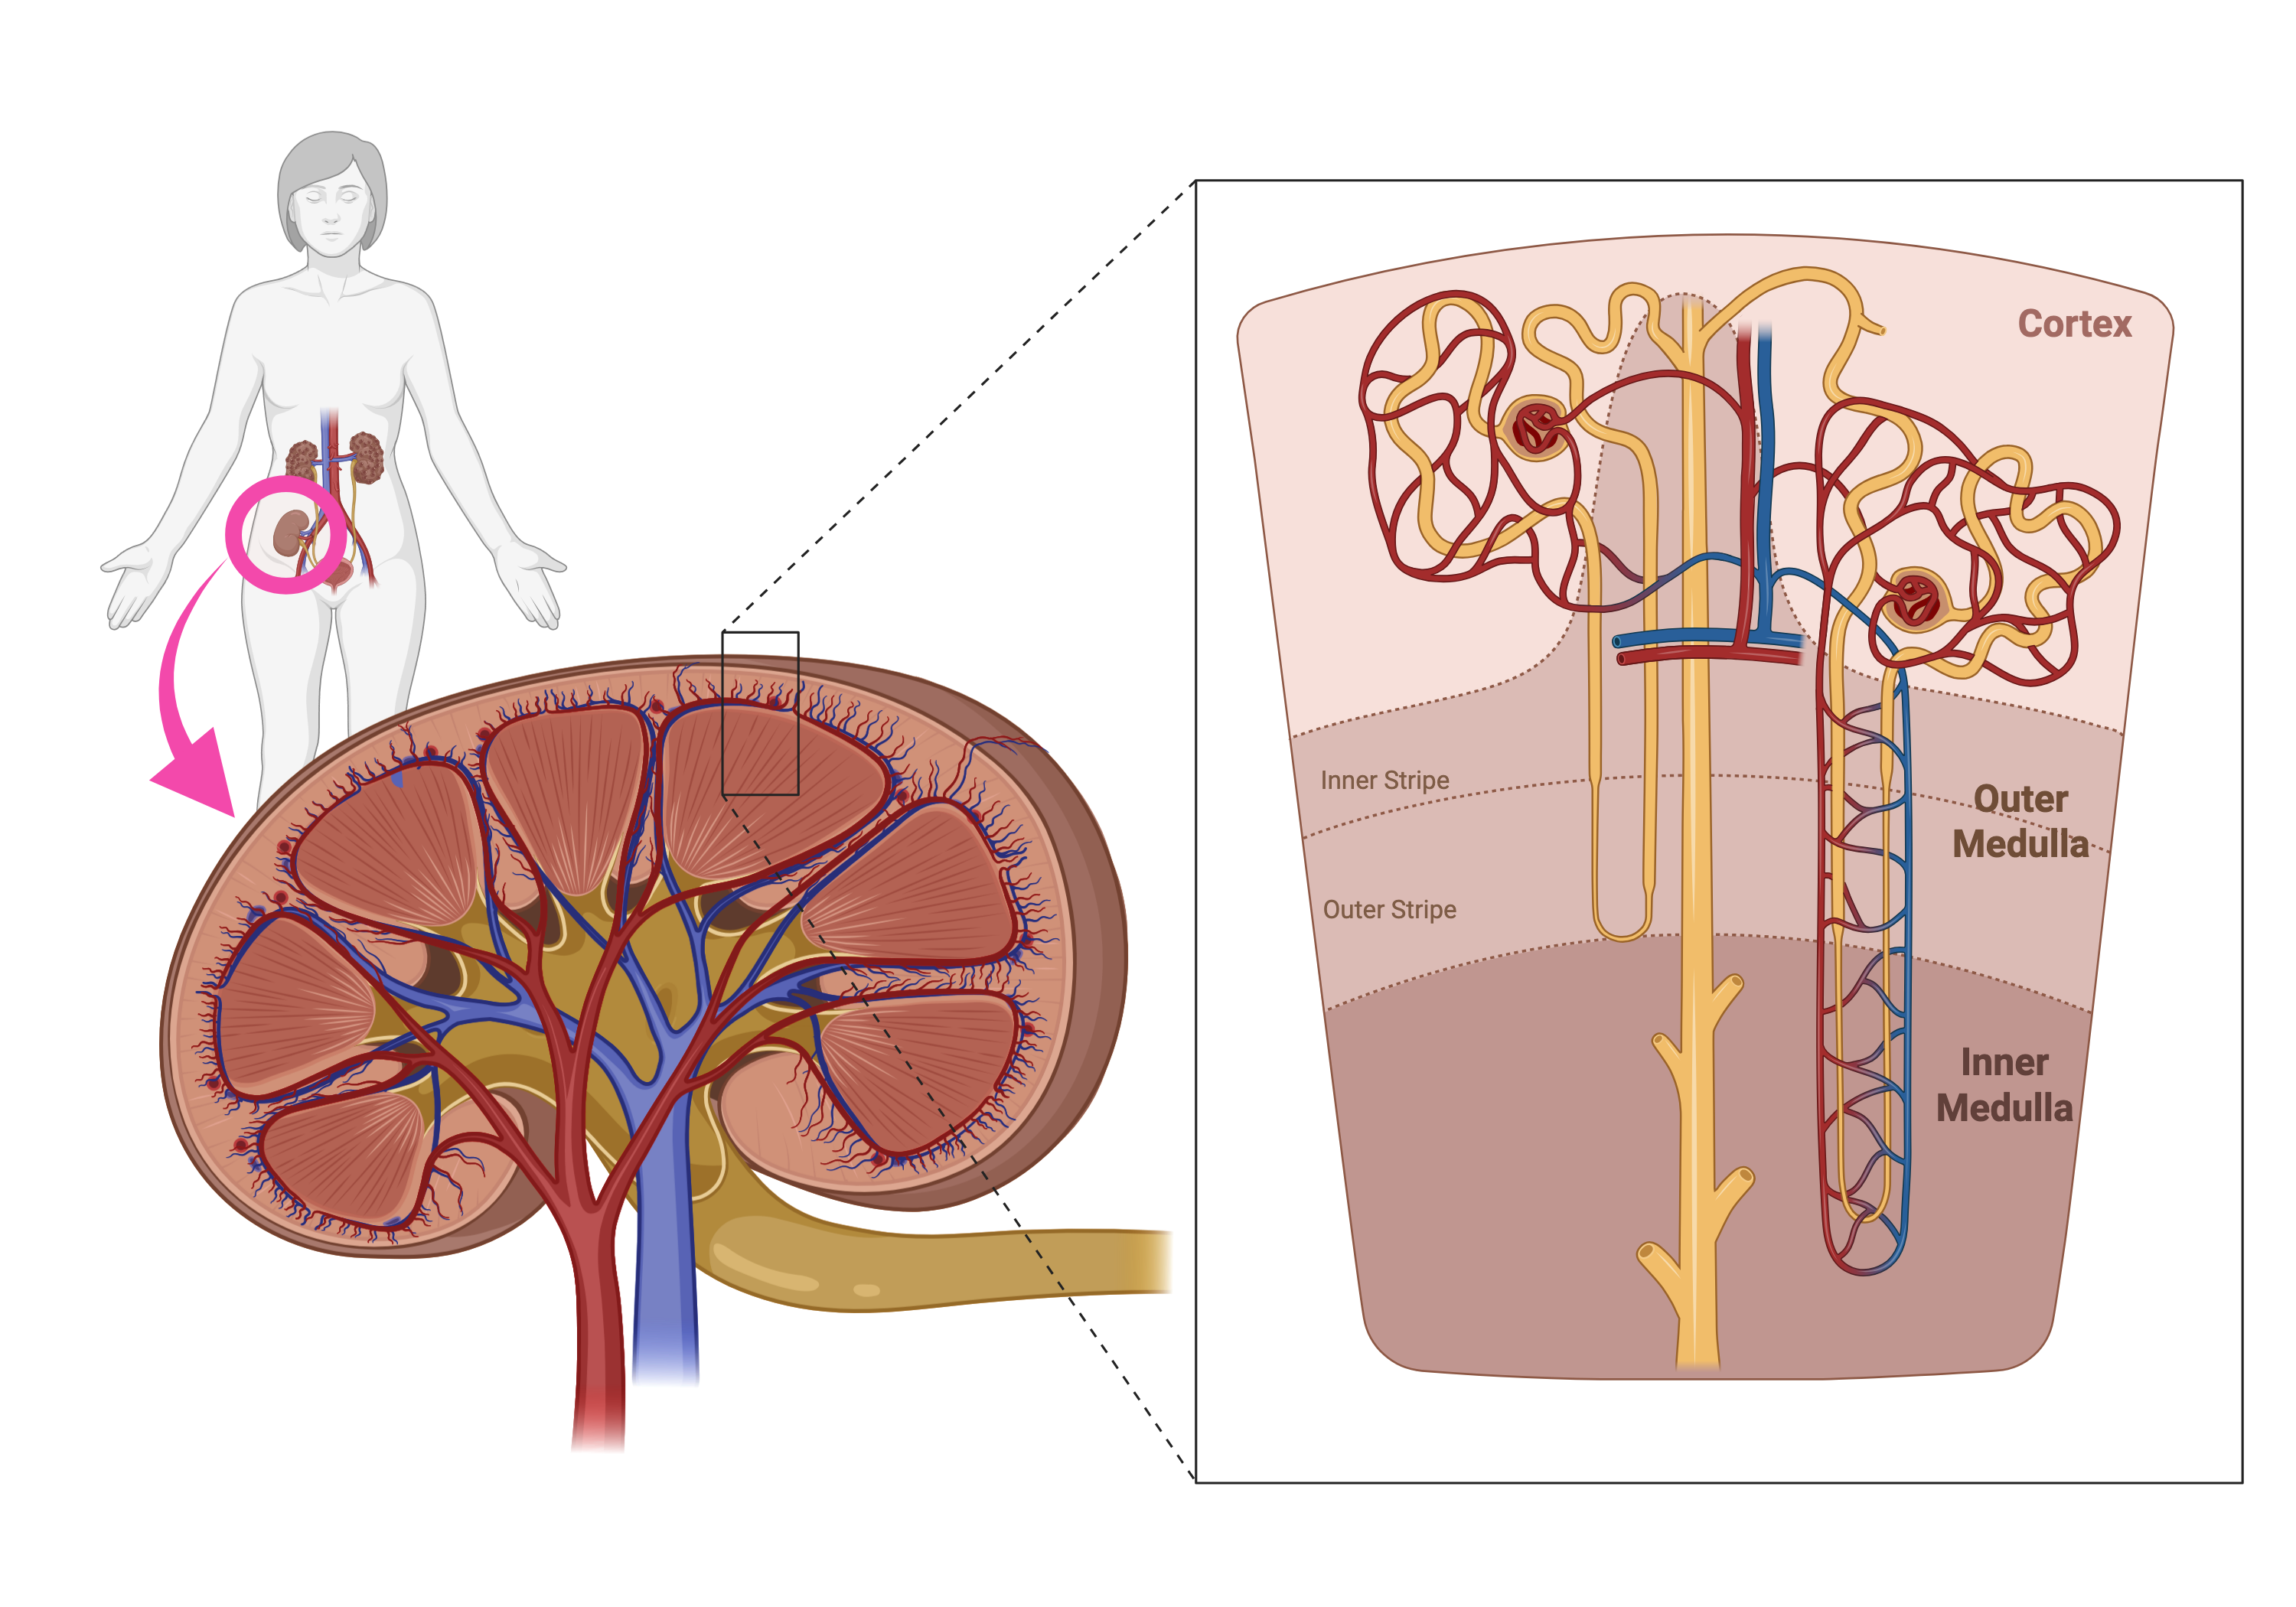
\includegraphics[width=0.85\textwidth]{parts/intro/anatomy.png}
    \caption{Macrostructural (left) and microstructural anatomy of the transplanted human kidney, with the site of a typical graft site (superficially in the anterior lower abdomen) circled in magenta. The left side shows the triangular-shaped medulla radiating out of the renal pelvis, surrounded by the cortex. The right side highlights the microstructure of the nephrons, as well as their relationship to the macroscopic features of the renal parenchyma, collecting system, and vasculature. Image created using BioRender.}
    \label{fig:anatomy}
\end{figure}

% Paragraph 2: nephrons are the functional units
%   - start in glomerulus (in cortex)
%   - proximal tubule (cortex)
%   - loop of Henle (medulla)
%   - distal tubule (cortex)
%   - collecting duct (medulla)
%   - about 1 million nephrons per kidney
%   - glomeruli perform passive filtration
%   - tubules perform active filtration, reabsorption, secretion; more metabolically demanding

Nephrons are the functional units of the kidney. Each kidney contains roughly 2 million nephrons, each of which work to filter blood and produce urine~\cite{shringi_EndStage_2026,fattah_How_2019}. A nephron begins with the glomerulus, located in the cortex, where excess solutes are passively filtered out of the bloodstream. The filtrate (i.e. partially formed urine) then passes through a series of tubules: the proximal tubule (cortex), the loop of Henle (medulla), the distal tubule (cortex), and finally the collecting duct (medulla). Throughout this process, the tubules actively reabsorb essential substances back into the bloodstream and secrete waste products into the filtrate. This active filtration process is metabolically demanding, requiring significant energy expenditure by tubular cells. While nephrons span both the cortex and medulla, kidney allograft biopsies typically focus on sampling the cortex~\cite{tsai_Current_2016} despite the medulla's functional importance and involvement in relevant pathologies~\cite{lopez_normal_2015,nankivell_Importance_2020,wei_Architecture_2015}.

% Paragraph 3: microvasculature supports nephrons
%   - glomerular capillaries
%   - afferent arteriole
%   - efferent arteriole
%   - peritubular capillaries
%   - vasa recta

The kidney's microvasculature plays a vital role in supporting nephron function. Blood enters the glomerulus through the afferent arteriole, where it is filtered by the glomerular capillaries. The filtered blood then exits via the efferent arteriole, which branches into the peritubular capillaries that surround the tubules, facilitating reabsorption and secretion processes. In the medulla, the vasa recta, a series of straight capillaries, help maintain the concentration gradient necessary for urine concentration.

% Paragraph 4: interstitial space holds it all together
%   - provides structural support
%   - mediates signaling between nephrons and vasculature
%   - ECM composition varies between cortex and medulla
%   - contains resident immune cells

Finally, the interstitial space within the renal parenchyma provides structural support to the nephrons and vasculature. It mediates signaling between these components, facilitating communication that is essential for maintaining kidney function. The extracellular matrix (ECM) composition varies between the cortex and medulla, reflecting their distinct functional roles. Additionally, the interstitial space contains resident immune cells that contribute to the kidney's defense mechanisms against pathogens and injury.

\subsection{Understanding the Banff Classification System for Renal Allograft Pathologies}

% what microstructural pathologies can exist in renal graft rejection
%   - cell morphology changes defined by Banff criteria
%     - semi-quantitative
%     - biopsy-based
%     - categorical
%     - localized to small regions of interest
%   - histological features can be grouped by location/type - explain in text, as well as a table of Banff score categories grouped by:
%     - axis 1: location
%       - interstitium
%       - vasculature (arterioles, capillaries)
%       - tubules
%       - glomeruli
%     - axis 2: injury type
%       - inflammation (total inflammation, capillaritis, tubulitis etc.)
%       - fibrosis (interstitial, glomerulosclerosis etc.)
%       - morphological changes (tubular atrophy, basal membrane thickening etc.)
%       - C4d deposition is a special case
%     - some Banff scores don't fit neatly into these categories - e.g.:
%       - interstitial fibrosis and tubular atrophy (IFTA)
%       - IFTA with interstitial inflammation (i-IFTA)
%       - IFTA with tubular injuries (t-IFTA)
%       - polyomavirus load (pvl)
%   - briefly acknowledge debates around molecular interpretation of graft dysfunction, but focus on "larger-scale" pathologies

Renal allograft biopsies are evaluated by identifying and grading various microstructural pathologies according to the Banff criteria. These criteria provide a semi-quantitative, categorical classification system for assessing changes to cellular morphology that may be associated with graft rejection and other abnormalities. The Banff system defines a diagnostic algorithm for characterizing pathologies in needle biopsy samples of the renal cortex using 17 different categories of histological features~\cite{loupy_Banff_2020}. 15 of those categories are listed in Table~\ref{tbl:banff}, grouped together by anatomical location (interstitium, vasculature, tubules, glomeruli) and injury type (inflammation, fibrosis, morphological changes). Lesion scores are defined by the extent of involvement within the sampled cortical tissue, graded on an ordinal scale from 0 to 3. Specific scores for different lesions are used alongside other contextual evidence to substantiate diagnoses that are relevant to graft dysfunction~\cite{boor_Renal_2015}.

% !TeX root = ../../main.tex

\begin{landscape}
    \singlespacing
    \begin{longtable}{
        p{1.00in} 
        p{0.30in} p{1.05in} 
        p{0.30in} p{1.20in} 
        p{0.30in} p{1.20in} 
        p{0.30in} p{1.05in}}
        \caption{Banff Classification of Renal Allograft Pathologies Grouped by Relevance to Biomechanical Alterations Except for \emph{i-IFTA} and \emph{t-IFTA}.}\\
        \label{tbl:banff}\\
        % Header
        \toprule
        \multirow{2}{=}{\textbf{Changes in/due to...}} & 
        \multicolumn{2}{l}{\textbf{Interstitia}} & 
        \multicolumn{2}{l}{\textbf{Vasculature}} & 
        \multicolumn{2}{l}{\textbf{Glomeruli}} & 
        \multicolumn{2}{l}{\textbf{Tubules}} \\
            & 
        Name & 
        Definition & 
        Name & 
        Definition & 
        Name & 
        Definition & 
        Name & 
        Definition \\
        \midrule
        \endfirsthead
        \endhead
        % Footer
        \endlastfoot
        % Row group 1: inflammation
        \multirow[t]{2}{=}{\textbf{Inflammation}} & 
        \textit{i} & 
        Interstitial \mbox{Inflammation} & 
        \textit{v} & 
        Intimal Arteritis & 
        \multirow[t]{2}{=}{\textit{g}} & 
        \multirow[t]{2}{*}{Glomerulitis} & 
        \multirow[t]{2}{=}{\textit{t}} & 
        \multirow[t]{2}{*}{Tubulitis} \\
        % Row 2: additional row 1 for inflammation
            & 
        \textit{ti} & 
        Total \mbox{Inflammation} & 
        \textit{ptc} & 
        Peritubular \mbox{Capillaritis} &
            & 
            & 
            & 
            \\
        \hline
        % Row group 2: fibrosis
        \multirow[t]{3}{=}{\textbf{Fibrosis}} & 
        \multirow[t]{3}{=}{\textit{ci}} & 
        \multirow[t]{3}{=}{Interstitial Fibrosis} & 
        \textit{cv} & 
        Vasc. Fibrous Intimal Thickening & 
        \multirow[t]{3}{=}{\textit{cg}} & 
        \multirow[t]{3}{=}{Double Contours of Glom. Basal Membrane} & 
        \multirow[t]{3}{=}{\textit{ct}} & 
        \multirow[t]{3}{=}{Tubular Atrophy} \\
        % Row 4: additional row 1 for fibrosis
            & 
            & 
            & 
        \textit{ah} & 
        Arteriolar \mbox{Hyalinosis*} & 
            & 
            & 
            & 
            \\
        % Row 5: additional row 2 for fibrosis
            & 
            & 
            & 
        \textit{aah} & 
        Hyaline Arteriolar Thickening* & 
            & 
            & 
            & 
            \\
        \hline
        % Row group 3: other
        \textbf{Other} & 
            & 
            & 
        \textit{C4d} & 
        C4d Staining on PTC Endothelia or Medullary Vasa Recta & 
        \textit{mm} & 
        Mesangial \mbox{Matrix} Expansion* & 
        \textit{pvl} & 
        Polyomavirus Nephropathy \\
        \bottomrule
    \end{longtable}
    \par\vspace{0.5em}
    \noindent*: Lesion types with asterisks denote purely descriptive changes that are not used for classifying rejection types in the Banff system.
\end{landscape}


The Banff system includes six numbered categories of diagnoses for renal allograft pathologies. The categories include those that are focused on AMR (a majority of Category 2), TCMR (Category 4), and borderline TCMR (Category 3), as well as those that are not directly related to rejection (Categories 1 for normal findings or nonspecific changes, and Category 6 for non-rejection-related findings such as polyomavirus nephropathy). However, Category 5 is of special relevance to this work: interstitial fibrosis and tubular atrophy (IFTA). IFTA is a common finding in chronic graft dysfunction and is characterized by the presence of fibrosis in the interstitial space along with atrophy of the renal tubules. In fact, the two Banff lesion scores not mentioned in Table~\ref{tbl:banff}, inflammation in the presence of IFTA (\emph{i-IFTA}) and tubulitis in the presence of IFTA (\emph{t-IFTA}), uniquely depend on the presence of IFTA for their definition. These six diagnostic categories, with exception of Category 1 with non-IFTA findings, are not mutually exclusive; a single biopsy can receive multiple diagnoses if the relevant criteria are met. Therefore, findings like IFTA can be found on their own, but they can also co-occur with - and may even act as risk factors of poorer graft survival rates for - other diagnoses such as AMR or TCMR.

As the complex procedure for identifying and classifying these microstructural pathologies suggests, renal allograft dysfunction and rejection are multifaceted processes that can manifest through a variety of histological changes. Recent works have sought to better understand these processes by integrating molecular information with traditional histological assessments~\cite{bloom_CellFree_2017,sugi_Imaging_2019,goutaudier_Evaluation_2024}. While these molecular approaches can provide valuable insights into the underlying mechanisms of graft dysfunction, this dissertation aims to be more practically focused. Therefore, the discussion will primarily center around the larger-scale pathologies defined by the Banff criteria, particularly those related to inflammation and fibrosis, which are more directly relevant to clinical diagnostics and patient management.

\subsection{A Multi-Scale Perspective of Kidney Pathologies}

% - Paragraph 1: view renal parenchyma microstructure through biomechanics lens
%   - consider renal parenchyma as composite material made of multiple components
%   - nephrons (tubules + glomeruli) = functional core that essentially acts as load-bearing structures
%   - microvasculature (arterioles + capillaries) = cross-link network with roles in perfusion and nutrient delivery
%   - interstitial space (ECM + fibroblasts + immune cells) = matrix that supports other two components
%   - biological tissue is generally considered to be viscoelastic
%     - EXAMPLE: kidney tissue viscoelasticity from literature

To connect the microstructural pathologies defined by the Banff criteria to biomechanical properties that can be noninvasively assessed using ultrasound-based techniques, it is helpful to understand the renal parenchyma through a biomaterials lens. Considering that the renal parenchyma is primarily composed of orientationally organized nephrons, a dense microvasculature network, and a supportive interstitial matrix, one can reasonably interpret it as a fiber-reinforced composite material~\cite{karimi_Measurement_2017,gennisson_Supersonic_2012}. Specifically, the tubules of nephrons can be viewed as load-bearing structures that provide mechanical integrity to the tissue, while the microvasculature (glomeruli, peritubular capillaries etc.) acts as a cross-link network that distributes mechanical loads and facilitates nutrient delivery. The interstitial space, which houses the extracellular matrix, resident immune cells, and lymphatic features, serves as the matrix phase that binds the other two components together and maintains overall tissue structure. Biological tissues, including the renal parenchyma, are generally considered to exhibit viscoelastic behavior, meaning they display both elastic (solid-like) and viscous (fluid-like) responses to mechanical loading. Prior studies have characterized the viscoelastic properties of kidney tissue~\cite{karimi_Measurement_2017,liu_Effect_2017,pirsoltan_Investigation_2025,vasconcelos_Kidney_2024}, demonstrating that these properties can be influenced by various factors such as hydration status, temperature, and pathological changes. 

% - Paragraph 2: histological changes and viscoelastic changes can be related
%   - in that model...
%     - tubular injury = changes to structural integrity of nephrons
%     - vascular injury = changes to fiber-matrix relationship
%     - interstitial changes = changes to matrix material properties
%   - nephrons are oriented radially from cortex to medulla
%   - therefore, renal parenchyma can be considered transversely isotropic
%   - thus, histological changes may lead to changes in viscoelastic anisotropy
%   - problem can be inverted; detecting viscoelastic changes may provide insight into underlying histological changes

Within this framework, the various histological changes defined by the Banff criteria can be interpreted as alterations to the biomechanical properties of the renal parenchyma. For instance, tubular injuries such as tubular atrophy can be viewed as disruptions to the structural integrity of the nephrons, potentially leading to decreased stiffness and altered viscoelastic responses. Likewise, vascular injuries such as capillaritis and arteritis, may affect the fiber-matrix relationship within the tissue, influencing how mechanical loads are distributed and absorbed. Interstitial changes, such as interstitial inflammation and fibrosis, can modify the material properties of the matrix phase. Given that nephrons are oriented radially from the cortex to the medulla, the renal parenchyma can be considered to be transversely isotropic (TI) in three dimensions - that is, its mechanical properties differ along one axis (along nephrons) while it is isotropic in the two orthogonal axes (perpendicular to nephrons). Furthermore, as mentioned in Section~\ref{sec:anatomy}, the composition of the renal parenchyma varies between the cortex and medulla, suggesting that disease processes may also exhibit viscoelastic heterogeneity across anatomical regions. Consequently, histological changes that affect the microstructure of the renal parenchyma may lead to detectable alterations in its viscoelastic anisotropy and heterogeneity. This relationship, then, may be inverted: by noninvasively assessing changes in the viscoelastic anisotropy and heterogeneity of the parenchyma of renal allografts, it may be possible to infer underlying histological changes associated with graft dysfunction and rejection - be it AMR, TCMR, IFTA, or other pathologies defined by the Banff criteria.

\subsection{Implications for Ideal Diagnostic Approaches}

% - Paragraph 1: ideal diagnostic approach should noninvasively assess information about microstructure of renal parenchyma
%   - noninvasive imaging preferred over biopsy because:
%     - avoids risks associated with invasive procedures
%     - allows for more frequent longitudinal monitoring
%     - captures spatial heterogeneity of graft pathology
%     - reduces sampling error inherent in biopsies
%   - ideal imaging modality should provide information about:
%     - inflammation vs. fibrosis
%     - severity of microstructural changes
%     - spatial distribution of pathologies
%     - temporal progression of graft dysfunction
%   - biomechanical properties (e.g. viscoelasticity) may serve as useful biomarkers because they reflect underlying microstructural changes

It is crucial to recognize that the Banff criteria focuses on microstructural changes that are localized to small regions of interest within the renal cortex. As an organ that is heterogeneous both in terms of macrostructure and cellular phenotypes, the kidney can exhibit significant spatial variability in pathology. This heterogeneity poses challenges for biopsy-based assessments, as the sampled tissue may not fully represent the overall state of the graft. As such, an ideal adjunct to needle biopsies for monitoring renal allografts would be a noninvasive imaging modality capable of providing information about the microstructure of the renal parenchyma. Noninvasive imaging techniques offer several advantages over biopsies, including the ability to avoid risks associated with invasive procedures, facilitate more frequent longitudinal monitoring, capture spatial heterogeneity of graft pathology, and reduce sampling error inherent in biopsies. An ideal imaging modality should provide insights into key aspects of graft health such as the the presence of inflammation and fibrosis, the severity of microstructural changes, the spatial distribution of pathologies, and the temporal progression of graft dysfunction. Given that biomechanical properties like viscoelasticity are influenced by underlying microstructural changes, they may serve as useful biomarkers for noninvasively assessing graft health.

% - Paragraph 2: viscoelastic properties can provide biologically relevant information about tissue microstructure
%   - inflammation = cellular infiltration, edema, increased vascular permeability
%     - likely leads to decreased stiffness, increased viscosity
%   - fibrosis = excess ECM deposition, scar tissue formation
%     - likely leads to increased stiffness, decreased viscosity
%   - Banff criteria distinguishes AMR, TCMR etc. based on presence of inflammation, fibrosis, other lesions
%   - thus, identification of inflammation and/or fibrosis via mechanical properties may act as biomarkers for graft pathologies including rejection

Viscoelasticity measurements can provide biologically relevant information about tissue microstructure that may be indicative of specific pathological processes. For example, inflammation is characterized by cellular infiltration, edema, and increased vascular permeability, which can lead to decreased tissue stiffness and increased viscosity~\cite{kimondo_Mechanical_2024}. Conversely, fibrosis involves excess extracellular matrix deposition and scar tissue formation, typically resulting in increased stiffness~\cite{wenger_Mechanical_2007}. Furthermore, the Banff \emph{i-IFTA} score, or the combined presence of interstitial inflammation where IFTA is present, is a particularly pertinent indicator of graft dysfunction and survival~\cite{gago_Kidney_2012,nankivell_causes_2018}. Since the Banff criteria considers information about inflammation and/or fibrosis to distinguish between different types of graft pathologies such as AMR and TCMR, the ability to identify these conditions through changes in mechanical properties may serve as valuable biomarkers for diagnosing and monitoring kidney allograft health.

% - conclusion: an ideal approach to gaining insight into underlying microstructural changes associated with graft dysfunction and rejection involves noninvasive assessments of viscoelastic properties of renal parenchyma

In conclusion, an ideal approach to gaining insight into the underlying microstructural changes associated with graft dysfunction and rejection involves noninvasive assessments of the viscoelastic properties of the renal parenchyma such that inflammation and/or fibrosis may be distinguished. By leveraging the relationship between biomechanical properties and histological changes, such imaging techniques have the potential to enhance our ability to monitor graft health and improve patient outcomes.
